% Temporary manuscript: author review only. Do not edit the shared abstract/introduction.
% !TeX program = latexmk
% Chinese review manuscript; English master and submission source: dp_puzzle.tex.
% Engine and output directory are set by .latexmkrc (XeLaTeX, build/).
\RequirePackage[T1]{fontenc}
\documentclass[conference,10pt,letterpaper]{IEEEtran}
\usepackage[no-math]{fontspec}
\usepackage{xeCJK}
\setmainfont{TeX Gyre Termes}
\setsansfont{TeX Gyre Heros}
\setmonofont{TeX Gyre Cursor}
\setCJKmainfont{FandolSong-Regular.otf}[
  BoldFont=FandolSong-Bold.otf,
  ItalicFont=FandolKai-Regular.otf,
  ItalicFeatures={FakeSlant=0.15},
  SmallCapsFont=FandolSong-Regular.otf]
\setCJKsansfont{FandolHei-Regular.otf}[BoldFont=FandolHei-Bold.otf]
\setCJKmonofont{FandolFang-Regular.otf}
\usepackage{amsmath,amssymb}
\usepackage{graphicx}
\usepackage[caption=false,font=footnotesize]{subfig}
\usepackage{booktabs}
\usepackage{cite}
\usepackage[hidelinks]{hyperref}
\graphicspath{{figures/}}


\newcommand{\PaperTitle}{DP-Puzzle: Exploring Multi-Precision Throughput Ratios in Tensor Cores through Composable Dot-Product Units}
\title{\PaperTitle}
\author{\IEEEauthorblockN{Anonymous Submission}}
\hypersetup{
  pdfauthor={},
  pdftitle={\PaperTitle},
  pdfsubject={Chinese working draft}}

\newcounter{DACreferencepage}
\AtEndDocument{%
  \ifnum\value{page}>\value{DACreferencepage}\relax
    \PackageWarningNoLine{DAC2027}{References exceed one page}%
  \fi}

\begin{document}
\bstctlcite{DPBSTcontrol}
\maketitle

% !TeX root = ../main.tex
\begin{abstract}
多精度张量计算单元通常采用 $1:2:4$ 的 16、8、4 位峰值算力配比。模型计算向低精度迁移后，增加低精度算力的收益同时取决于硬件成本和工作量组成。本文提出 DP-Puzzle，通过组合共享全精度 Group 与 Q、E、QE 专用 Group 构建九种点积单元配比，覆盖工业界已有选择及更大的增配空间。基于 12\,nm、1\,GHz 下的综合面积和真实负载活动功耗，建立由基准阵列面积占比与功耗预算倍率共同约束的整核部署模型，将单 DP 成本映射为分精度绝对算力。结果表明，$1:2:8$ 的 E 算力翻倍仅增加 33.60\% 的 DP 面积，而 $1:4:8$ 的 Q/E 同时翻倍增加 68.21\%；更大的增配还受到可配置核数的限制。以 DeepSeek-V4.1-Flash 为主要负载，构造 11 个上下文与 32 个算子精度方案，用最坏相对损失评价固定芯片。基准面积占比 30\%、DP 功耗预算为基准 1.5 倍时，原始精度下选择 $1:4:4$，跨上下文最坏损失为 3.91\%；覆盖全部迁移方案时选择 $1:4:8$，最坏损失为 20.05\%。该方法将可组合微架构、双预算成本和精度迁移联系起来，为算力配比选择提供依据。
\end{abstract}
\begin{IEEEkeywords}
多精度算力配比，组合式点积单元，张量计算，面积功耗约束，设计空间探索
\end{IEEEkeywords}


% !TeX root = ../main.tex
\section{引言}
\label{sec:introduction}
%%下面的文字内容，仅支持小范围的文本描述修改优化，不允许大范围重写
随着大模型技术的发展，模型的参数规模与计算需求持续增长，采用更低精度的数值格式已成为常见的优化手段~\cite{deepseekv3}。通用矩阵乘法（GEMM）作为大模型的主要计算负载，其计算格式也逐渐由单精度浮点格式（FP32）向低精度格式拓展。其中，最主要的代表包括 TensorFloat-32（TF32）、半精度浮点格式（FP16）和 BF16。随着大模型量化技术的发展，FP8、INT8、FP6、FP4，以及引入共享缩放因子（scaling factor）的微缩放（Microscaling）格式~\cite{ocpmx2023}，也逐渐成为模型推理优化中的重要选择。以 DeepSeek-V4.1-Flash~\cite{deepseekv41source}为例，其文本主干采用按算子配置的混合精度策略：混合专家（MoE）计算及多数注意力投影采用 FP8；稀疏注意力索引器的 QK 路径采用 MXFP4；主注意力的 QK/PV 计算采用 BF16。因此可见，当前大语言模型推理呈现出了多种精度计算需求并存的特点，对承载大模型推理的硬件也带来了更高的要求。

在硬件设计方面，在相同的数据输入位宽下，低精度格式可同时传入更多元素，形成BF16:MXFP8:MXFP4之间$1:2:4$的峰值算力配比。但是，当前工业界的最新AI芯片也逐渐打破这种传统的模式，通过定向提高FP4算力，或同时增强FP8与FP4的峰值算力，来增强产品竞争力。但是模型的发展的节奏与芯片设计制造周期的之间有较大差异,根据当前的模型需求设计芯片可能无法满足未来的发展变化。因此芯片设计必须为未来的模型负载变化留有设计余量。从AI芯片的主要算力来源——张量计算单元（Tensorcore）来分析，需要在支持多种计算精度的基础上，还需要对不同精度之间的相对算力进行取舍，留有计算容量，兼顾当前与未来的下模型发展需求，并权衡由此带来的硬件成本和收益。

因此针对模型负责变化选择合适的芯片算力配比，这一极具工程价值和实际意义的问题，我们提出了DP-Puzzle ,将算力配比选择的硬件成本与模型负载收益联系起来。由于Tensorcore的设计中，通常采用点积单元结合脉动~\cite{jouppi2017tpu}或者广播的数据传输格式，构建二维计算阵列。因此针对算力配比问题，我们以点积单元为主要的算力配比改变的硬件设计实现，支持多种数据精度格式的计算，支持改变低精度的算力。根据真实的面积功耗硬件成本，作为算力配比分析的基础。结合硬件成本和模型负载收益，分析不同模型负载迁移下的不同算力配比的综合收益，为芯片设计配比的规格定义提供参考依据。

% BEGIN INLINE TABLE: related_features
% Promoted from the approved temporary manuscript.
\suppressfloats[t]
\begin{table}[t]
\centering
\caption{精度支持与组合式配比配置能力。}
\label{tab:related_features}
\begingroup\footnotesize\setlength{\tabcolsep}{1pt}
\def\Y{$\checkmark$}\def\N{$\times$}\def\E{$\triangle$}
\begin{tabular*}{\columnwidth}{@{\extracolsep{\fill}}l*{10}{c}@{}}\toprule
Design & TF32 & FP16 & BF16 & \shortstack{MX\\FP8} & \shortstack{MX\\FP6} & \shortstack{MX\\FP4} & INT8 & \shortstack{NV\\FP4} & HiF4 & \shortstack{Multi\\Ratio} \\\midrule
Ten-Four~\cite{rout2026tenfourv3} & \Y & \Y & \Y & \Y & \N & \N & \Y & \N & \N & \N \\
MXDOTP~\cite{islamoglu2025mxdotp} & \N & \N & \N & \Y & \N & \N & \N & \N & \N & \N \\
FPnew~\cite{mach2021fpnew} & \N & \Y & \Y & \E & \N & \N & \N & \N & \N & \N \\
MiniFloats~\cite{bertaccini2024minifloats} & \N & \Y & \Y & \E & \N & \N & \N & \N & \N & \N \\
TransDot~\cite{transdot2026} & \N & \Y & \N & \E & \N & \E & \N & \N & \N & \N \\
\midrule
DP-Puzzle & \Y & \Y & \Y & \Y & \Y & \Y & \Y & \Y & \Y & \Y \\
\bottomrule\end{tabular*}
\par\smallskip
\parbox{\columnwidth}{\raggedright
$\checkmark$: supported; $\times$: absent in the reported configuration; $\triangle$: element arithmetic supported, integrated MX scaling not established. FPnew and MiniFloats also support FP32/FP64; MiniFloats uses FP8 E5M2/E4M3 and BF16-encoded FP16alt.}
\endgroup
\end{table}

% END INLINE TABLE: related_features
本文的主要贡献如下：
\begin{enumerate}
\item \textbf{可组合的多精度点积微架构。} 我们提出 DP-Puzzle，采用 Lane、Group 和点积单元三级架构，支持 TF32、FP16/BF16、INT8、MXFP8/6/4、NVFP4 和 HiF4。设计在不同精度间复用乘法、对齐与规约资源，并通过增配专用 Group 独立扩展低精度吞吐。
\item \textbf{九种算力配比的实现与评估。} 我们实现九种 BF16:MXFP8:MXFP4 峰值算力配比，覆盖基线、三种产业配比及五种扩展配置，并基于 12\,nm 逻辑综合与负载驱动功耗分析量化其实现成本。相较于 \mbox{$1:2:4$}，\mbox{$1:2:8$} 将 MXFP4 吞吐翻倍，面积增加 33.60\%，MXFP4 面效和能效分别提高 49.70\% 和 27.27\%。
\item \textbf{联合预算下的配比选择。} 我们在相同总核心面积和点积阵列功耗预算下，估算各配比的可部署核心数与分精度峰值算力。在 DeepSeek-V4.1-Flash prefill 的五种精度迁移场景和 11 个上下文长度的综合评估中，\mbox{$1:2:8$} 在九种配比中表现最佳，相对 \mbox{$1:2:4$} 取得 $1.13\times$ 的理想 GEMM 计算加速。
\end{enumerate}

本文其余部分安排如下：第~\ref{sec:background}~节介绍背景与动机；第~\ref{sec:architecture}~节阐述组合式点积微架构与配比构造；第~\ref{sec:evaluation}~节给出评估方法及面积、功耗结果；第~\ref{sec:workload}~节分析面积、功耗约束与精度负载迁移下的配比选择；第~\ref{sec:conclusion}~节总结全文。


% !TeX root = ../main.tex
\section{背景与动机}
\label{sec:background}

\subsection{浮点精度与微缩放格式}
\label{sec:formats}

BF16/FP16 由逐元素的指数与有效数确定动态范围和精度~\cite{burgess2019bfloat16}；微缩放格式则将低位宽元素与共享尺度共同编码（图~\ref{fig:fpformats}）。OCP MXFP8/6/4 每 32 个元素共享一个 E8M0 尺度~\cite{ocpmx2023}；NVFP4 使用 16 元素一组的 E4M3 尺度~\cite{nvidia2024nvfp4}；HiF4 使用 64 元素一组的无符号 E6M2 基础尺度，并为每 8、4 个元素分别配置一位微指数~\cite{hifloat4}。元素编码、分组粒度和尺度编码分别决定解包、局部规约与尺度融合的硬件需求。

\begin{figure}[t]
\centering
\includegraphics[width=\columnwidth]{fp_format.png}
\caption{元素编码与共享尺度~\cite{ocpmx2023,nvidia2024nvfp4,hifloat4}。字段标注为位宽，$g$ 为缩放组大小。}
\label{fig:fpformats}
\end{figure}


\subsection{张量计算与点积单元}
\label{sec:tensor_organization}

对于矩阵乘累加 $D=C+AB$，$M$、$N$ 是输出维度，$K$ 是归约维度。点积单元先对齐多个乘积并集中归约，再统一规格化和舍入，以共享后端摊薄逐项浮点处理的成本~\cite{lutzFusedFP84Way2024}。本文采用 H 类原生归约长度为 16 的 DP 作为基线，与已有数值建模研究识别的点积累加粒度相对应~\cite{xie2025mmasim}。完整 GEMM 沿归约维拆为多笔请求，单 DP 接收显式 $C$ 并输出 $D$，跨请求部分和保存在其外部。

有无组尺度的格式可用同一局部点积结构描述。依据 OCP 的点积定义，共享尺度可提出组内归约~\cite{ocpmx2023}。将 $L$ 项乘积按缩放组边界划分为 $G=\lceil L/g\rceil$ 组，末组不足部分补零，加入累加输入 $c$ 后，有
\begin{equation}
d=c+\sum_{j=0}^{G-1}X_j^{(A)}X_j^{(B)}
\underbrace{\sum_{i=0}^{g-1}P_{j,i}^{(A)}P_{j,i}^{(B)}}_{q_j}.
\label{eq:blockdot}
\end{equation}
其中，$X_j^{(A)}$、$X_j^{(B)}$ 为两路输入第 $j$ 组的共享尺度，$P_{j,i}^{(A)}$、$P_{j,i}^{(B)}$ 为组内元素的解码值，$q_j$ 为组内点积；HiF4 的局部微指数计入元素解码。对于无组尺度的格式，令 $X_j^{(A)}=X_j^{(B)}=1$，即可得到普通点积累加。

式~\eqref{eq:blockdot} 给出分层共享的算术边界；内部位宽、顺序与舍入仍由具体实现约束。



\subsection{通路复用与设计空间探索}
\label{sec:datapath_sharing}

表~\ref{tab:related_features} 汇总格式与组合能力。MX 列区分完整微缩放支持与仅元素运算支持；本文通过在共享 DP 内增配专用 Group 改变算力配比。

已有工作通过跨精度共享降低单元成本：TransDot 重组乘法器与移位器~\cite{transdot2026}，MPICC 将多种格式映射为统一内部表示~\cite{huangMPICCMultiplePrecisionInterCombined2025}，融合 FP8 点积设计复用累加和舍入后端~\cite{lutzFusedFP84Way2024}。DSE 研究进一步联合探索数值格式与 MAC 微架构~\cite{paretomac2025}，或共享尺度、权重和激活格式~\cite{zhao2026mxlike}；Timeloop 则以循环分块与存储层次分析阵列映射~\cite{timeloop2019}。本文固定目标格式集合，将 H/Q/E 峰值配比作为设计变量，考察实测单元成本如何通过面积与功耗预算影响部署规模与负载收益。

\subsection{算力配比的设计动机}
\label{sec:commercial_ratios}
\label{sec:ratio_motivation}

表~\ref{tab:vendor_ratios} 展示了从 $1:2:4$ 向 E 增强或 Q/E 同时增强的产品与研发路线。已有选择给出了配比变化的方向，但不能覆盖不同负载和硬件预算下的全部选择。本文进一步考察只增强 Q、提高 E 增配幅度以及扩大 Q/E 共同增配的组合，将 $1:4:4$、$1:2:12$、$1:2:16$、$1:6:12$ 和 $1:8:16$ 纳入探索，与上述四种配比共同构成九候选设计空间。



更高的低精度峰值需要额外乘法、对齐和规约资源，也会改变整核面积和逐模式功耗。因此，配比选择需要同时回答：单位成本能增加多少低精度吞吐，以及面积与功耗预算允许配置多少核心。本文以组合式微架构构造候选，以同工况测量建立成本，再将预算决定的绝对算力映射到 H/Q/E 负载组成，分析工业界已有选择和更大增配方案各自的优势区域。


% !TeX root = ../main.tex
% 本章按当前规格、CModel 与 Verilog 核验；英文稿按作者后续要求同步。
\section{面向配比探索的组合式点积微架构}
\label{sec:architecture}
\label{sec:brick_definition}

DP-Puzzle 采用 Lane、Group 与 DP 三层组合式架构（图~\ref{fig:dp_architecture}）。Lane 共享元素乘法与局部归约，Group 融合缩放因子并输出统一表示的部分和，DP 完成全局对齐、累加与输出处理。设计的核心是以统一的 Group 接口连接多精度共享通路与低精度专用通路：保留完整格式支持，通过增配专用 Group 调整各精度的峰值算力，同时共享末端累加、规格化与舍入。九种配置的硬件资源在设计阶段确定，运行时按请求切换计算精度。

\subsection{符号与记号约定}
\label{sec:notation_conventions}

本文以 T、H、Q、E 表示四类精度：T 为 TF32，H 为 FP16/BF16，Q 为 MXFP8（E4M3/E5M2）与 MXFP6（E2M3/E3M2），E 为 MXFP4、NVFP4 与 HiF4。后文用这些简称描述各类精度的计算通路与算力配比。

定点数采用 $\mathrm{Q}I.F$ 与 $\mathrm{UQ}I.F$ 记号：$I$ 为不含符号位的整数位数，$F$ 为小数位数~\cite{ti2003qformat}。$\mathrm{Q}I.F$ 表示二进制补码有符号数，总位宽为 $1+I+F$；$\mathrm{UQ}I.F$ 表示无符号数，总位宽为 $I+F$。例如，UQ2.26 为含 2 位整数与 26 位小数的 28 位无符号数。

计算并行度记为 $\mathrm{T}x_T\mathrm{H}x_H\mathrm{Q}x_Q\mathrm{E}x_E$，各下标变量表示对应模式每周期处理的 A/B 元素对数，每对产生一个乘积。例如，T1H2Q4E8 表示 T/H/Q/E 模式每周期分别计算 1/2/4/8 个乘积。各精度模式互斥，上述数值不能相加作为同时可用的吞吐。一个 Lane 支持 T1H2Q4E8，两个 Lane 构成一个 Group，四个 Group 构成 T8H16Q32E64 基线；每个 Lane 另支持四路 INT8 乘法，DP 支持 INT32 累加。各配置均采用八级流水，每拍接收一笔独立请求。

对于固定的 $m\times n$ DP 阵列，精度 $p$ 的原生点积长度为 $K_p$，时钟频率为 $f$。当每拍均有输入且阵列充分利用时，峰值算力为
\begin{equation}
\mathrm{Peak}_p=2mnK_pf\quad(\mathrm{FLOP/s}).
\label{eq:array_peak_throughput}
\end{equation}
一次 MAC 计为两次浮点运算，因此 $K_H:K_Q:K_E$ 直接决定同构阵列的峰值配比。后续设计通过改变低精度模式的 $K_p$ 构造候选，并分别表征其面积、功耗与供数开销。

\begin{figure}[t]
\centering
\includegraphics[width=\columnwidth]{baseline_arch_singlepage.pdf}
\caption{缩放粒度驱动的 Lane--Group--DP 划分。HiF4 每 8 个元素共享一个二级微指数，对应一个 Lane 的 8 路 E 类乘积；NVFP4 每 16 个元素共享一个尺度，对应两个 Lane 组成的 Group。更大的量化块向多个 Group 广播同一尺度，保持原格式的缩放粒度。}
\label{fig:dp_architecture}
\end{figure}

\subsection{Lane：跨精度共享与低精度定点化}
\label{sec:unpack_recode}
\label{sec:full_brick}

\textbf{统一解包与乘法复用。}图~\ref{fig:data_unpack} 给出各格式的内部表示。T/H 保留指数与有效数，Q 映射为内部 E5M3 表示；该映射通过指数调整和小数位补零保持原值。MXFP4/NVFP4 将元素指数融入 UQ3.1 幅值，HiF4 将一级微指数并入 UQ2.2 幅值。Lane 采用两组可复用的部分积单元：TF32/FP16 按位权组合部分积，Q/E 则将乘法叶子用于独立的低精度乘积，避免为每种格式复制完整乘法通路。

\begin{figure}[t]
\centering
% 图稿待作者统一数量标签：按完整 Lane 标注时，FP16 为 2x，E 为 8x；
% 右侧 10/16/4 位描述单个字段组，每个 Lane 包含两个字段组。
\includegraphics[width=\columnwidth]{unpack_layout.png}
\caption{各格式到共享计算字段的映射。Q 统一指数与有效数表示，E 将元素指数或一级微指数融入定点幅值；符号与特殊值状态独立传递。}
\label{fig:data_unpack}
\end{figure}

\textbf{按精度组织对齐与归约。}T/H/Q 使用组内共同的最大乘积指数，通过四路共享右移器完成局部对齐，幅值窗口为 UQ2.26。E 类在解包后采用固定坐标，无需逐元素指数比较与宽移位：八个乘积先两两合并，再接入共享的四路归约树。HiF4 的二级微指数由 Lane 部分和之后的小范围移位消化，避免引入跨 Lane 的 E 类指数对齐。由此，低精度计算可以复用乘法与加法资源，同时旁路高精度所需的对齐通路。

\subsection{Group：规约后尺度融合与统一部分和}

\textbf{将尺度运算移至组内规约之后。}两个 Lane 共享同一组尺度，Group 先合并其部分和，再对幅值施加两侧尺度有效数的乘积。NVFP4/HiF4 共用一套 $14\times8$ 无符号乘法器，处理 14 位组幅值与 8 位尺度有效数乘积；MX 的幂次尺度仅计入指数。尺度乘法由此按 Group 执行，无需在每个元素乘积上重复计算。物理 Group 的划分不改变量化块大小，同一量化块的尺度按需广播到多个 Group。

\textbf{分离数值坐标与幅值处理。}各类 Group 统一输出符号、31 位幅值及指数信息。令幅值为 $\mathrm{SoP}$、位宽为 $M$、符号为 $s$，原始坐标 $\mathrm{Anchor}$ 表示幅值最高物理位的指数，则有限组结果的数值为
\begin{equation}
v=(-1)^s\mathrm{SoP}\,2^{\mathrm{Anchor}-(M-1)}.
\label{eq:anchor_recompute}
\end{equation}
Anchor 由局部乘积指数、尺度指数及格式相关的定点布局修正提前计算，与幅值归约并行。对有限非零部分和，前导零检测仅产生比较指数 $e=\mathrm{Anchor}-\operatorname{LZC}_M(\mathrm{SoP})$，不在 Group 内移动幅值。该接口既保留原始数值坐标，又为后端提供实际最高有效位的指数，使不同专用 Group 能共用同一对齐与累加通路。

\subsection{DP：一次净移位与共享融合累加}

累加项 $C$ 在组内规约和尺度融合之后才加入全局指数比较与累加，避免其指数提前影响 E 类的局部定点计算。Group 使用经前导零校正的指数 $e$；$C$ 使用解码后的有效指数，保留 FP32 非正规数的指数约定，不做前导零校正。有限非零参与源共同确定全局参考 $E_{\max}$，零值与特殊值不参与数值 MAX。

每路原幅值低位补零至 39 位窗口后，按净移位量 $\Delta=\mathrm{Anchor}-E_{\max}$ 执行一次双向移位：正值左移，负值右移并向零截断。该操作将 Group 的前导零规格化与全局对齐合并，无需先移动幅值再重新对齐。恢复符号后，各路进入 carry-save 压缩网络，最后通过一次进位传播加法得到总和。中间部分和不转为 FP32，仅在最终输出时规格化并采用最近偶数舍入。INT8 复用乘法资源，与 INT32 累加项共用末端加法通路，旁路浮点对齐和输出规格化舍入。

\subsection{低精度专用 Group}
\label{sec:specialized_midgroups}

专用化保留统一的 Group 输出接口，并按目标精度裁剪解包、乘法、对齐和寄存器，而非只改变输入格式选择。本文提供三类可组合单元。

\textbf{E 专用单元。}E8 Lane 仅保留低精度解包、八个 $4\times4$ 乘法器及窄归约树，HiF4 的局部微指数在 Lane 内完成融合。两个 Lane 构成 E16 Group，复用组级尺度乘法，补零后接入公共部分和接口。该路径无需 T/H/Q/INT8 的解码、元素指数比较与宽对齐逻辑。

\textbf{Q/E 共享单元。}Q4E8 Lane 以八个 $4\times4$ 乘法器支持两类精度：Q 模式启用四个，E 模式启用全部八个。两个 Lane 构成 Q8E16 Group；Q 保留指数比较与宽对齐，E 旁路对齐并复用归约和尺度处理。因而 QE 增配仍需承担 Q 的宽对齐与规约成本，不能按 E 专用单元的成本线性放大。

\textbf{Q 专用单元。}Q4 Lane 与 Q8 Group 仅保留 Q 的乘法、指数对齐及归约，删除 E 相关的配对、微指数与尺度有效数乘法，用于单独提高 Q 吞吐。三类专用单元分别支持 E 定向增配、Q/E 共同增配与 Q 定向增配。

\subsection{DP 内算力配比配置}
\label{sec:expansion}

四个多精度 Group 构成 T8H16Q32E64 基线。在此基础上增加 2、4、8、12 个 E16 Group，分别得到 $1:2:6$、$1:2:8$、$1:2:12$、$1:2:16$；增加 4 个 Q8 Group 得到 $1:4:4$；增加 4、8、12 个 Q8E16 Group，分别得到 $1:4:8$、$1:6:12$、$1:8:16$。连同 $1:2:4$ 基线，共形成九种全精度配比，均保留 TF32、FP16/BF16 与 INT8 通路。

新增 Group 计算同一输出的额外 A/B 片段，与基础 Group 使用统一的全局参考指数，在 carry-save 网络内合并部分和。全局 MAX、各源对齐移位器和规约网络随组数扩展；$C$ 只加入一次，最终进位传播加法器、规格化与舍入仍保持单份。网络末端按请求精度选择基础或扩展后的两行，再送入唯一的进位传播加法器，避免在分支合并之前引入串联的进位传播。累加位宽随源数增长，保留对齐后各项求和所需的增长位。

各配置均保持八级流水与 II=1。扩展组按对应请求的精度更新寄存器，非参与组从指数比较、数值累加及特殊值归约中屏蔽。该组织使算力配比成为设计阶段的可组合参数，并将各候选的成本差异落实到专用前端、扩展对齐和规约资源，为后续面积、功耗与部署规模的联合分析提供基础。


% !TeX root = ../main.tex
\section{算力配比的硬件成本表征}
\label{sec:evaluation}

\subsection{实验设置与验证}
\label{sec:eval_setup}
\label{sec:numerical_validation}

九种点积单元以 Verilog 实现，使用 Synopsys Design Compiler X-2025.06 在 TSMC 12\,nm 工艺、TT（0.7\,V、85$^\circ$C）工况下以 1\,GHz 综合，启用集成时钟门控，并通过时序与电气检查。面积统计包含组合逻辑、流水寄存器和门控单元。

功耗评估采用 Qwen3-8B 在 WikiText-2 上运行时第一层 MLP 下投影的激活与权重~\cite{qwen3technicalreport,merity2016pointer}，分别量化为 BF16、MXFP8 E4M3 和 MXFP4 E2M1。Power Compiler 基于 1\,GHz 门级仿真提取的稳态开关活动估计总功耗。面积与功耗均对应综合后、CTS/布局布线前的单 DP。精度验证采用真实模型负载的多精度量化数据，结合随机及边界向量，通过 Verilator 对每种配置完成覆盖 11 种格式的 10,747 笔测试。以独立的精确二进制算术模型为参考，完整计算包含块缩放与累加项 $C$ 的点积，仅在最终结果处按最近偶数舍入至 FP32。在受测数据上，BF16 的最大误差为 3 个 FP32 ULP，其余浮点格式不超过 1\,ULP，其中 HiF4 为 0；INT8/INT32 精确匹配。

\subsection{基线设计与同类多精度单元比较}
\label{sec:related_dp_evaluation}

% Promoted from the approved temporary manuscript.
\suppressfloats[t]
\begin{table}[t]
\centering
\caption{精度支持与组合式配比配置能力。}
\label{tab:related_features}
\begingroup\footnotesize\setlength{\tabcolsep}{1pt}
\def\Y{$\checkmark$}\def\N{$\times$}\def\E{$\triangle$}
\begin{tabular*}{\columnwidth}{@{\extracolsep{\fill}}l*{10}{c}@{}}\toprule
Design & TF32 & FP16 & BF16 & \shortstack{MX\\FP8} & \shortstack{MX\\FP6} & \shortstack{MX\\FP4} & INT8 & \shortstack{NV\\FP4} & HiF4 & \shortstack{Multi\\Ratio} \\\midrule
Ten-Four~\cite{rout2026tenfourv3} & \Y & \Y & \Y & \Y & \N & \N & \Y & \N & \N & \N \\
MXDOTP~\cite{islamoglu2025mxdotp} & \N & \N & \N & \Y & \N & \N & \N & \N & \N & \N \\
FPnew~\cite{mach2021fpnew} & \N & \Y & \Y & \E & \N & \N & \N & \N & \N & \N \\
MiniFloats~\cite{bertaccini2024minifloats} & \N & \Y & \Y & \E & \N & \N & \N & \N & \N & \N \\
TransDot~\cite{transdot2026} & \N & \Y & \N & \E & \N & \E & \N & \N & \N & \N \\
\midrule
DP-Puzzle & \Y & \Y & \Y & \Y & \Y & \Y & \Y & \Y & \Y & \Y \\
\bottomrule\end{tabular*}
\par\smallskip
\parbox{\columnwidth}{\raggedright
$\checkmark$: supported; $\times$: absent in the reported configuration; $\triangle$: element arithmetic supported, integrated MX scaling not established. FPnew and MiniFloats also support FP32/FP64; MiniFloats uses FP8 E5M2/E4M3 and BF16-encoded FP16alt.}
\endgroup
\end{table}

% Generated by scripts/build_related_native.py; official manuscript.
\begin{table*}[t]
\centering
\caption{已有单元与 DP-Puzzle 的原工艺实现条件及效率。}
\label{tab:related_dp}
\begingroup\footnotesize\setlength{\tabcolsep}{1.5pt}
\def\Eff#1{\begin{tabular}{@{}lr@{}}#1\end{tabular}}
\begin{tabular*}{\textwidth}{@{\extracolsep{\fill}}l*{8}{c}@{}}\toprule
Metric & Ten-Four~\cite{rout2026tenfourv3} & MPICC~\cite{huangMPICCMultiplePrecisionInterCombined2025} & MXDOTP~\cite{islamoglu2025mxdotp} & FPnew~\cite{mach2021fpnew} & MiniFloats~\cite{bertaccini2024minifloats} & TransDot~\cite{transdot2026} & \multicolumn{2}{c}{DP-Puzzle} \\
\cmidrule(lr){8-9}
 & & & & & & & $1:2:4$ & $0:2:4$ \\
\midrule
Structure & Fused DP & $n$-term MAC & MX DP & SIMD FMA & SIMD wDotp & FMA / DP & MX DP & MX DP \\
Technology (nm) & 7 & 28 & 12 & 22 & 12 & 12 & 12 & 12 \\
Voltage (V) & 0.7 & 0.9 & 0.8 & 0.8 & 0.8 & 0.8 & 0.7 & 0.7 \\
Frequency (GHz) & 1.58 & 1.43 & 1.09 & 0.923 & 1.26 & 1.0 & 1.0 & 1.0 \\
Area ($\mu$m$^2$) & 2400 / 4650 & 2295 & 3150 & 49\,000 & 19\,000 & $\approx 6000^\dagger$ & 16\,165.12 & 11\,695.21 \\
Accumulation & FP32/INT32 & FP12/INT8 & FP32 & Per format & FP16/FP32 & FP32 & FP32/INT32 & FP32 \\
\midrule
\shortstack[l]{Energy efficiency\\(TFLOP/s/W)} & --- & \Eff{FP8 & 1.948\\FP4 & 5.931} & \Eff{MXFP8 & 2.035} & \Eff{FP16 & 0.498\\BF16 & 0.582\\FP8 & 1.245} & \Eff{FP8 & 1.63\\FP16 & 0.82} & \Eff{FP16 & 0.556\\FP8 & 1.190\\FP4 & 2.439} & \Eff{BF16 & 2.088\\MXFP8 & 4.000\\MXFP4 & 11.432} & \Eff{MXFP8 & 4.713\\MXFP4 & 12.527} \\
\midrule
\shortstack[l]{Area efficiency\\(TFLOP/s/mm$^2$)} & \Eff{BF16 & 5.250 / 5.419\\MXFP8 & 10.500 / 10.839} & \Eff{FP8 & 1.246\\FP4 & 4.985} & \Eff{MXFP8 & 5.524} & \Eff{FP16 & 0.151\\BF16 & 0.151\\FP8 & 0.303} & \Eff{FP8 & 1.06\\FP16 & 0.53} & \Eff{FP16 & $\approx 0.67^{\dagger}$\\FP8 & $\approx 1.33^{\dagger}$\\FP4 & $\approx 2.67^{\dagger}$} & \Eff{BF16 & 1.980\\MXFP8 & 3.959\\MXFP4 & 7.918} & \Eff{MXFP8 & 5.472\\MXFP4 & 10.945} \\
\bottomrule\end{tabular*}
\par\smallskip
\parbox{\textwidth}{\raggedright
均为原工艺数据，不做工艺归一化；支持范围见表~\ref{tab:related_features}。Ten-Four 为全格式 Q8/Q16；MiniFloats 取独立 wDotp FPU，非 cluster。
$\dagger$：TransDot 面积由原文图 7(a) 的 1\,ns 点估读，面效按表 II 吞吐计算；原文相对其 12\,nm FPnew 基线的平均 FP16/FP8 面效为 1.46$\times$/2.92$\times$，不与本表 22\,nm FPnew 值相乘。--- 表示无报告值或不适用。}
\endgroup
\end{table*}


表~\ref{tab:related_features} 与表~\ref{tab:related_dp} 分别比较格式覆盖与实现效率。本文选取 $1:2:4$ 基线作为完整多精度设计的代表，支持 TF32、FP16/BF16、MXFP8/6/4、NVFP4、HiF4 及 INT8，浮点与整型运算分别采用 FP32 和 INT32 累加。相比表中已有单元，该设计在共享通路中覆盖更完整的低精度块缩放格式，兼容 MXFP8/6/4、NVFP4 和 HiF4，并支持多种算力配比，为不同量化方案提供统一的计算基础。

各项效率采用原文报告的工艺与测量条件，以下重点比较同为 12\,nm 的实现。相对 MiniFloats，本文基线的 FP8 面效与能效分别为其 $3.74\times$ 和 $2.45\times$；相对 TransDot，FP8 对应约 $2.97\times$ 和 $3.36\times$，FP4 对应约 $2.97\times$ 和 $4.69\times$。其中，TransDot 的面积由原图估读，相关面效及倍率为近似值，表中以 $\dagger$ 标识。结果表明，完整多精度覆盖与块缩放支持能够兼顾较高的面积和能量效率。

针对采用 7\,nm 工艺的 Ten-Four，表中保留原始数据，正文另用 DeepScaleTool~\cite{sarangi2021deepscaletool} 作工艺缩放比较，以其支持的 14\,nm 节点作为本文 12\,nm 的近似参照。将面积与延迟分别放大 $7.273\times$ 和 $1.132\times$ 后，其全格式 Q8/Q16 配置的 MXFP8 面效估计为 1.275/1.316\,TFLOP/s/mm$^2$，本文 $1:2:4$ 基线为其 $3.10\times$/$3.01\times$。该比较为工艺缩放估算。

针对仅支持低精度计算模式，我们同时列出 $0:2:4$ 低精度专用点积单元设计，以展示格式专用化的收益：在保持 Q32E64 并行度的同时，移除其他精度支持，使 MXFP8 面效由 3.959 提高至 6.555\,TFLOP/s/mm$^2$，能效由 4.000 提高至 5.230\,TFLOP/s/W。按各自原工艺与测量条件比较，相对同为 12\,nm 的 MXDOTP，其 MXFP8 面效提高 18.67\%，能效为其 $2.57\times$，并增加 MXFP4、NVFP4 和 HiF4 支持。相对 28\,nm 的 MPICC，FP8 面效与能效分别为其 $5.26\times$ 和 $2.68\times$，FP4 分别为 $2.63\times$ 和 $2.35\times$。采用上述工艺缩放方法，相对 Ten-Four 的 MXFP8 专用 Q8/Q16 配置，本文 $0:2:4$ 的 MXFP8 面效分别为其 $2.15\times$/$2.10\times$，同时保留 FP4 计算支持。

\subsection{九种配比的面积与功耗}
\label{sec:lowp_costs}

图~\ref{fig:ratio4_costs} 给出九种配比的面积与总功耗，面积倍率以 $1:2:4$ 为参照，功耗直接报告 mW。以下各模式增幅均与基线的同精度功耗比较。$1:2:6$ 和 $1:2:8$ 分别将 E 算力提高 50\% 和 100\%，DP 面积仅增加 16.69\% 和 33.60\%，E 模式功耗增加 28.77\% 和 57.14\%。两者的 H/Q 模式功耗增幅均低于 4\%，表明共享后端与按模式激活能够限制增配资源对其他精度的影响。

$1:4:8$ 将 Q/E 算力同时翻倍，面积增加 68.21\%；Q 和 E 模式功耗分别增加 79.91\% 和 83.66\%，H 模式仅增加 2.71\%。其 Q 模式总功耗为 28.789\,mW。与 E 专用增配相比，QE Group 还需保留 Q 的指数比较、局部对齐及宽规约通路，因而具有更高成本。

更大增配进一步展开了成本差异。$1:2:12$ 和 $1:2:16$ 将 E 容量提高至基线的 3 倍和 4 倍，面积分别增加 64.68\% 和 83.68\%，E 功耗增加 109.56\% 和 162.42\%。只增强 Q 的 $1:4:4$ 面积增加 48.56\%，低于共同增配的 $1:4:8$。$1:6:12$、$1:8:16$ 的面积增幅分别为 136.52\% 和 190.29\%，Q 模式功耗达到 41.351 和 52.853\,mW；九种配置的 H 功耗增幅均不超过 6.27\%。

\begin{figure*}[t]
\centering
{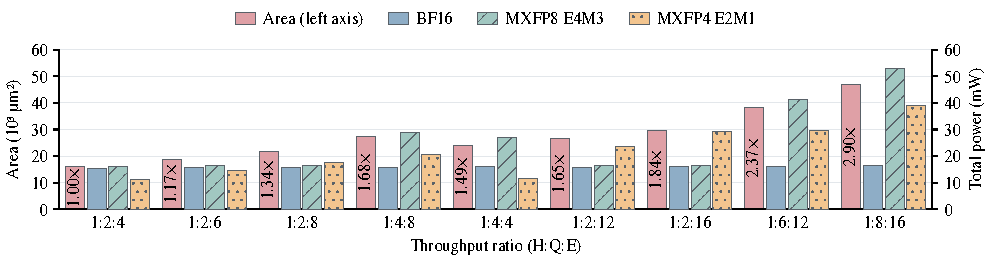
\includegraphics[width=2\columnwidth]{dp_ratio_area_power.pdf}}
\caption{九种配比的综合面积与总功耗。面积柱按左轴读取，标签为相对 $1:2:4$ 的倍率；三种精度的功耗柱按右轴读取（mW）。}
\label{fig:ratio4_costs}
\end{figure*}

\textbf{观察一：算力、面积与功耗不按同一比例增长。} E 专用通路能以较小成本提高 E 吞吐，而同时提高 Q 吞吐需要更多对齐与规约资源。因此，配比 DSE 应使用各候选的面积和逐模式功耗，不能按峰值比例线性放大基线成本。

\subsection{持续供数所需的带宽}
\label{sec:ratio_bandwidth}

考虑固定的 $m\times n$ DP 阵列：A 沿行广播并在本地寄存器中复用 $x$ 个周期，B 沿列广播且每周期更新。每个 DP 每拍处理 $K$ 项乘积，频率为 $f$，同一精度下每元素占 $b$ 位（含均摊尺度开销），则 shared memory 向阵列提供输入的稳态平均带宽需求为
\begin{equation}
B_{\mathrm{in}}(K,x)=fbK\left(\frac{m}{x}+n\right),\qquad
\frac{B_{\mathrm{in}}(K_j,x)}{B_{\mathrm{in}}(K_0,x)}=\frac{K_j}{K_0}.
\label{eq:ratio_bandwidth}
\end{equation}
这里固定阵列尺寸、频率及复用周期，并假设完整缩放块下输入位数随 $K$ 同比增长。A 的复用降低了重复读取开销，但每周期更新的 B 仍需持续供给。因此，相比 $1:2:4$，$1:2:8$ 的 E 模式、$1:4:8$ 的 Q/E 模式在满吞吐下均需要约两倍输入带宽。增配低精度算力时，需要同时考虑 shared memory 的供给是否跟得上阵列消费；后续 DSE 仍以供数充分为前提，不加入 shared memory 带宽约束。


% BEGIN independent DSE draft; compact fixed-budget analysis, 2026-11-16.
% Temporary manuscript only. The author promotes accepted text to the official manuscript.
\section{面积与功耗约束下的算力配比探索}
\label{sec:workload}

\subsection{从单 DP 成本到整核部署}
\label{sec:k4_area}

以 $1:2:4$ 为基准，每个 SM 配置 $D=256$ 个 DP，基准部署 $N_0=36$ 个 SM。令 $a_j$ 为候选 $j$ 的单 DP 面积，$\alpha$ 为基准计算阵列占 SM 的面积比例。固定每核外围面积 $A_O$，共同面积预算为
\begin{equation}
A_O=Da_0(\alpha^{-1}-1),\qquad A_{\mathrm{bud}}=N_0Da_0/\alpha.
\end{equation}

以 $p_{j,p}$ 表示 H/Q/E 模式的单 DP 测量功耗，取 $p_j^{\max}=\max_p p_{j,p}$。共同 DP 功耗预算为 $P_{\mathrm{bud}}=\beta N_0D p_0^{\max}$，实际部署数量由两项预算共同决定：
\begin{equation}
n_j=\min\!\left\{
\left\lfloor\frac{A_{\mathrm{bud}}}{A_O+Da_j}\right\rfloor,
\left\lfloor\frac{P_{\mathrm{bud}}}{Dp_j^{\max}}\right\rfloor
\right\}.
\label{eq:core_area_budget}
\end{equation}
同一候选的物理核心数在精度和上下文之间保持不变，所有已配置核心均满足各模式的功耗上限。取 $f=1$\,GHz、II=1，模式 $p$ 的原生点积长度为 $K_{j,p}$，则峰值算力及充分供数下的计算时间为
\begin{equation}
C_{j,p}=2fDn_jK_{j,p},\qquad T_j(L,z)=\sum_p\frac{F_p(L,z)}{C_{j,p}}.
\end{equation}
$F_p(L,z)$ 是上下文 $L$、精度场景 $z$ 下的 GEMM 工作量，各精度阶段顺序执行。主比较固定 $\alpha=0.3$、$\beta=1$，对应共同面积预算 496.59\,mm$^2$ 和 DP 计算池功耗上限 147.47\,W。

\subsection{固定预算下的精度迁移收益}

\begin{figure*}[!t]
\centering
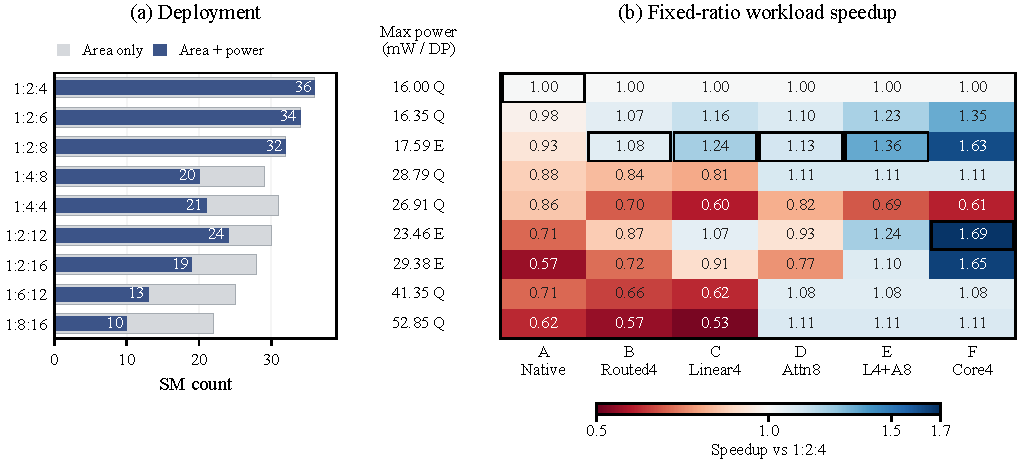
\includegraphics[width=\textwidth]{temp/dse_fixed_budget.pdf}
\caption{同面积、同功耗上限下的九配比比较，$\alpha=0.3$、$\beta=1$。(a) 灰条为仅面积约束核数，蓝条及数字为双约束实际核数；中列为单 DP 三模式最大功耗及对应模式 Q/E。(b) 每个候选在全部上下文采用固定部署，数值为同精度场景下 baseline 与候选平均计算时间之比，黑框表示各列平均时间最短的候选。A--F 为正文定义的精度迁移场景；各上下文等权，1.00 表示与 $1:2:4$ 相同。}
\label{fig:fixed_budget_compact}
\end{figure*}

采用 DeepSeek-V4.1-Flash~\cite{deepseekv41source} 的冷启动 prefill，batch=1，上下文从 1K 至 1M 逐次翻倍，共 11 点。A 保持原始精度；B 将路由专家转为 FP4；C 在 B 上将共享专家和 Q-up/O-up 转为 FP4；D 从 B 分支，将主注意力 QK/PV 与 Grouped O-down 转为 FP8；E 合并 C/D；F 将 E 中的主注意力与 Grouped O-down 进一步转为 FP4。其余算子保持原精度，FP32 工作单列。对上下文计算时间等权求均值，报告 $S_j(z)=\overline T_0(z)/\overline T_j(z)$，每个场景内的配比不随上下文改变。

\textbf{发现一：相同 FP4 单元容量下，非对称增配可保留更高部署密度。}
$1:2:8$ 与 $1:4:8$ 的单 DP E 吞吐相同，但最大模式功耗分别为 17.59\,mW（E）与 28.79\,mW（Q），预算内分别部署 32 和 20 个 SM，前者整芯片 E 算力高 60\%。Q 模式的功耗要求会约束同一设计在 E 模式下的部署规模，因此 Q/E 同时增配不一定适合 E 密集负载。

\textbf{发现二：适度的非对称增配能在不增加预算的条件下兑现精度迁移收益。}
原始场景 A 由 $1:2:4$ 取得最低平均时间；在 B、C、E 中，$1:2:8$ 分别达到 baseline 的 1.08、1.24、1.36 倍计算性能。C 中其平均性能亦为 $1:4:8$ 的 1.53 倍，且在全部上下文相对 baseline 均获得 1.18--1.26 倍加速。进一步迁移到 F 时，$1:2:12$ 以 1.69 倍加速取得优势。负载迁移决定增配方向，双预算下的部署密度决定适宜的增配幅度。

\textit{作者补充：确认 C--F 的模型质量可行范围，以及目标芯片外围功耗与实际矩阵利用率。}
% END independent DSE draft.


% !TeX root = ../main.tex
\section{结论}
\label{sec:conclusion}

本文围绕当前与未来混合精度负载的算力配比选择，提出组合式多精度点积微架构 DP-Puzzle，构建九种共享后端的配比设计。12\,nm、1\,GHz 下，$1:2:8$ 相比 $1:2:4$ 将 MXFP4 吞吐翻倍，面积增加 33.60\%，面效与能效分别提高 49.70\% 和 27.27\%，体现了精度专用增配与通路共享的收益。

联合面积、功耗与精度负载迁移的探索表明，高功耗模式会通过压缩部署规模影响其他精度的收益。在基准 TensorCore 面积占比 30\%、相同面积与 DP 池功耗预算下，$1:2:8$ 比 $1:4:8$ 提供高 60\% 的整芯片 FP4 算力，并在 DeepSeek-V4.1-Flash 的 1K--1M 上下文与六场景等权评测中取得最低平均计算时间，相对基线的加速比为 1.147 倍。该理想计算结果说明，保留部署密度与高精度算力的适度增配，能够适应多种低精度迁移路径；固定芯片的配比应由实现成本与跨负载收益共同决定。


\section*{Content Generated by AI}
本研究使用 OpenAI Codex 辅助 EDA 脚本生成、源码与微架构说明梳理，以及实验建模、数据分析、图表脚本和全文结构与文字草稿的整理。作者对采用的脚本、结果及全部论述承担责任。



\clearpage
\setcounter{DACreferencepage}{\value{page}}
\ifnum\value{DACreferencepage}>7\relax
  \PackageWarningNoLine{DAC2027}{Main text exceeds six pages}%
\fi
\typeout{DAC2027: References start on page \thepage}
\bibliographystyle{IEEEtran}
\bibliography{references/references}

\end{document}
